\section{Using RF Noise as True Random Number Generator} \label{Seed}

PRNGs require an unpredictable seed, i.e. a true random number as a starting point. Higher end devices, such as security ICs hence come with a dedicated true random number generator. The CC2538 manual does not claim that using RF noise is a suitable source for random numbers in a cryptographic context, however, in the absence of another source, developers are bound to use what is available. The CC2538 User's Guide\cite{CC2538Manual} explains to fill the SOC\_ADC\_RNDL register with random bits from the Intermediate Frequency Analogue-to-Digital Converter (IF\_ADC) in the RF receive I/Q channels to seed the PRNG (Section 16.2.2). The user guide\cite{CC2538Manual} also reports on the good quality of the randomness (Section 23.12). 

%\cite{CC2538Manual}:
%\begin{quote}
%For the CC2538, when a random value is required, writing the SOC\_ADC\_RNDL register with random bits from the IF\_ADC in the RF receive path seeds the LFSR.
%\end{quote}
%and also: (Section 23.12 in CC2538 User's Guide\cite{CC2538Manual})
%\begin{quote}
%Single random bits from either the I or Q channel can be read from the RFRND register.
%\end{quote}

%We note that the Contiki driver only uses the bits generated in I channel. 

%\begin{quote}
%Randomness tests show good results for this module. However, a slight DC component exists. In a simple test where the RFRND.IRND register was read a number of times and the data was grouped into bytes, about 20 million bytes were read. When interpreted as unsigned integers between 0 and 255, the mean value was 127.6518, which indicates that there is a DC component.
%...
%For the first 20 million individual bits, the probability of a 1 is $P(1) = 0.500602$ and $P(0) = 1 - P(1) = 0.499398$.
%\end{quote}

%Their test results are shown in \Cref{SeedResult}.

%\begin{figure}[!t]
%\centering
%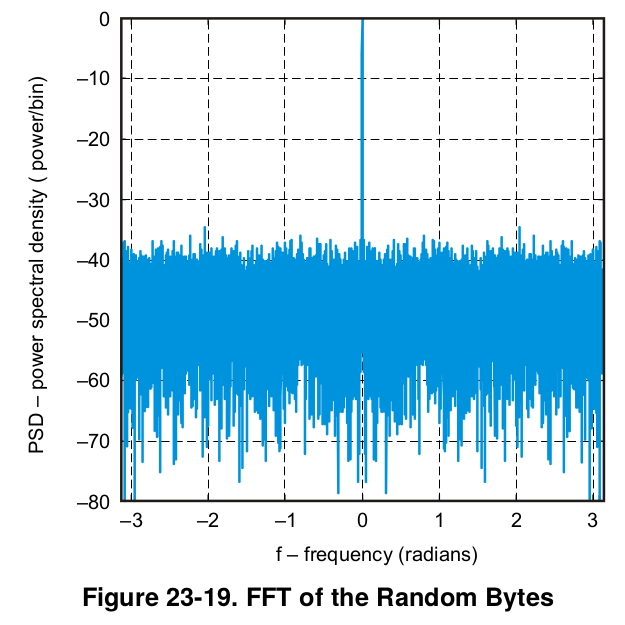
\includegraphics[width=2.5in]{fig/CC2538_Seed1.png}
%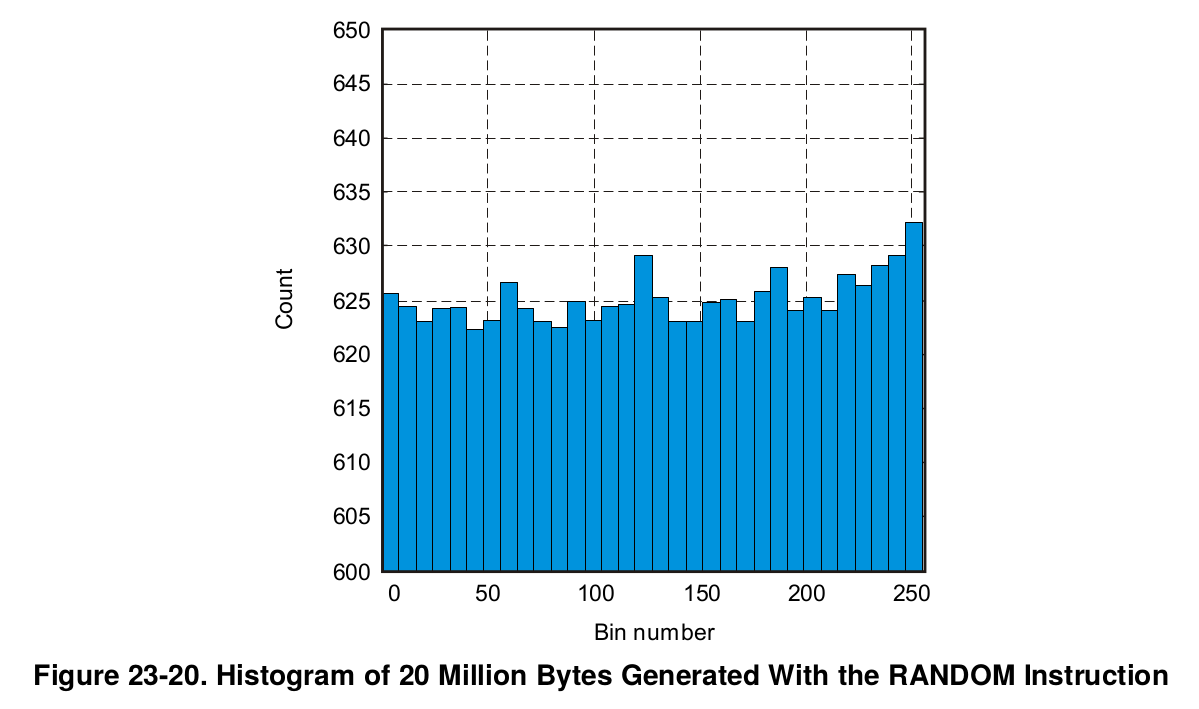
\includegraphics[width=2.5in]{fig/CC2538_Seed2.png}
%\caption{RF core seeding result, from CC2538 User's Guide}
%\label{SeedResult}
%\end{figure}

To verify the claims in the manual, we applied the NIST Statistical Test Suite\cite{NISTTest} on 13263600 bits sampled by this seeding method. Since one bit is returned upon each read to the RNG register, we concatenated all bits into one bit stream. The bits passed all tests in the NIST test suite, with $P(0) = 0.49995001$ and $P(1) = 0.50004999$, which shows that the RF noise (when not tampered with) is indeed a good source for random numbers. However, it remains unclear whether such source can practically be influenced by crafted RF signals. %The full report and raw data are applicable at \cite{prngtest}.

%Despite the good randomness of the seed, sampling from RF noise remains sceptical from a security perspective as such physical source could be tampered remotely by sending jamming signal to the device.

\subsection{Reverse Engineering the TRNG Design}
The documents supplied by TI do not explain further details of how IF\_ADC in the receive I/Q channels are translated to random bits. We have neither been able to find any open document describing the RF design of CC2538. However, we noticed that the same design has been applied to several products in TI's SimpleLink\texttrademark series, some of which provided a better explanation of their RF core and RNG designs. 

\begin{figure}[!t]
\centering
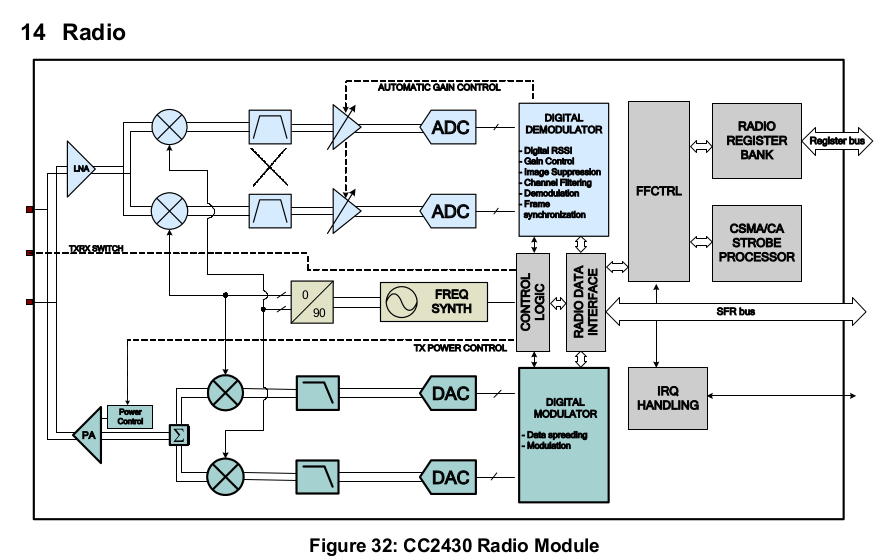
\includegraphics[width=2.5in]{fig/CC2430_Radio.png}
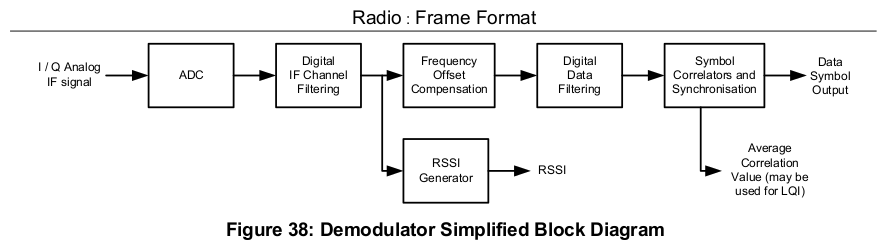
\includegraphics[width=2.5in]{fig/CC2430_Demodulator.png}
\caption{CC2430 RF Design, from CC2430 user manual\cite{CC2430Manual}}
\label{CC2430RF}
\end{figure}

In the CC2430 user manual\cite{CC2430Manual}, we found a description of its RF core as in \Cref{CC2430RF} which explains that the input analogue signal to IF\_ADC goes through the following components:

\begin{itemize}
	\item Low Noise Amplifier (LNA) which amplifies the signal.
	\item Mixer which down converts the signal frequency. The Frequency Synthesiser is used as the local oscillator.
	\item Band pass filter which removes the out of band signals.
	\item The Automatic Gain Control (AGC) circuit further adjusts the signal strength to the input level of ADC.
\end{itemize}

The CC2520 Data Sheet\cite{CC2520Manual} explains the random bit is actually the LSB from ADC output: (Section 24 in CC2520 Data Sheet\cite{CC2520Manual})
\begin{quote}
Single random bits from either the I or Q channel (configurable) can be output on GPIO pins at a rate of 8MHz. One can also select to xor the I and Q bits before they are output on a GPIO pin. These bits are taken from the least significant bit in the I and/or Q channel after the decimation filter in the demodulator.
\end{quote}

A block diagram is also provided, as shown in \Cref{CC2520RFRND}.
\begin{figure}[!t]
\centering
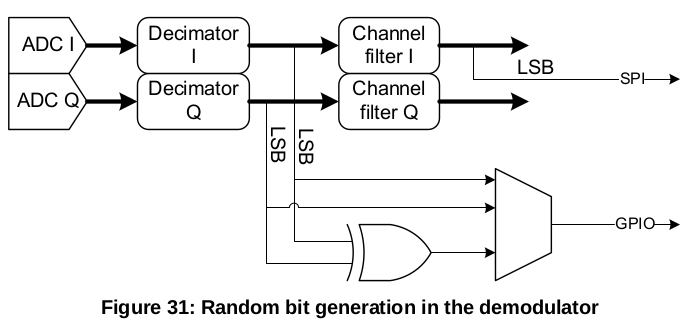
\includegraphics[width=2.5in]{fig/CC2520_RNG.png}
\caption{CC2520 RNG Design, from CC2520 user manual\cite{CC2520Manual}}
\label{CC2520RFRND}
\end{figure}

Interestingly, we noticed that CC2538, CC2520, CC253X and CC2540/41 reported exactly the identical randomness test result in their user manuals (\cite{CC2538Manual} \cite{ CC2520Manual} \cite{CC2530Manual}). We suspect the above evidence showed that CC2538 is very likely to have adopted the same designs.

The designs above explained the nice randomness of the seeding method. Denote $V_s$ as the analogue RF signal and $N$ as the noise, the analogue input to the ADC, denote as  $V_{in}$, can be represented as:
\begin{equation} \label{V_in}
V_{in} = V_s + N
\end{equation}

The noise $N$ can be induced by multiple sources in practice, including noise produced by the signal source, environmental noise, and noise induced by the components in the device itself, etc.

The random bit $b$ can therefore be represented as:
\begin{equation} \label{RNDOutput}
b = LSB(V_{in}) = LSB(V_s + N)
\end{equation}
where $LSB() \in \{0,1\}$ represents the operation of taking the LSB of A/D conversion output.

From \Cref{RNDOutput} we observe that any difference in $V_{in}$ that is larger than the scale of ADC, i.e. the voltage represented by the LSB of ADC, could flip $b$. According to the CC2538 Datasheet\cite{CC2538Datasheet}, the receiver can be sensitive to signals down to $-97dBm$ (typical value with $T_A = 25^{\circ}C$, $V_{DD} = 3V$ and $f_{C} = 2440MHz$). On the other hand, the typical environmental noise in our experimental environment is about $-92dBm$ which is significantly higher than the receiver sensitivity. We consider this reading as a generic office use case and the result of randomness test  as evidence to the sampling method.

\section{Biasing the RF Signal in Practice}\label{Jamming}
 \Cref{RNDOutput} indicates that the random bit $b$ is jointly determined by the signal $V_s$ and noise $N$. Although an adversary can generate arbitrary signals, i.e. $V_s$ is fully  controlled by the adversary, it is clear that controlling $N$ is difficult in practice. For instance, noises accumulated by different amplification stages are physically inevitable and intrinsic to the physical device. Hence it is not straightforward to fully control $V_{in}= V_s +N$ in practice.

An alternative attempt is to provide the RF with an `illegal' input $V_{in}$. We considered two methods in our experiments: saturation and decimation. Saturation attempts to provide the RF with a strong signal that is above its acceptance level, whereas decimation attempts to suppress any RF signal to beneath the receiver sensitivity.

Ideally we expect these illegal inputs will trigger the ADC into a fault state which could potentially results into a predictable ADC output and thus biased $b$. But in practice, decimation does not seem practical for the same reason that noise induced by the circuit itself is physically inevitable. This made saturation the only viable option for us. We further note that the undisclosed circuit design of the device also posed a difficulty in our experiments. Without knowledge of the exact circuit design, we had to perform black box experiments. 

\subsection{Concrete experiments}
We used OpenMote\cite{OpenMote}, a CC2538 powered SoC, for our experiments. %The receiver has been configured to $2475MHz$ (channel 25 in 802.15.4) which is the default value for CC2538 in Contiki. 
We extended the length of each seed from RF  to 128 bits in our experiments in coping to a potential PRNG design based on AES-128, although we still consider the bits are generated bitwise when applying the NIST test suite.

\subsection{Strong sine wave signal} \label{StrongSine}
The first signal we attempted was a strong sine wave signal. According to CC2538 data sheet\cite{CC2538Datasheet}, the saturation signal strength for the RF receiver is $10 dBm$. We have attempted to increase the input signal strength up to $13dBm$, which is roughly double of the saturation voltage, but no bias was observed. The seed sampled under this signal has passed all tests in the NIST test suite.

The result implies that the AGC circuit could have tuned down the signal which might have consequently prevented the seed from being biased. Although the exact AGC design for CC2538 is unclear, \Cref{AGC_QSL} demonstrates an example of AGC design using 4 Voltage Controlled Amplifiers (VGAs). The output signal is parallelly connected to a detector to estimate the signal strength. The output of detector is compared to a reference voltage and their difference is provided as a feedback to adjust the control voltage of VGAs. To prevent signal distortion caused by abrupt voltage change, such as during a lightning storm, many AGC design adopts an attack time (or called settle time) before it adjusts the gain. \cite{AGC} provides a detailed description of different AGC designs. 

\begin{figure}[!t]
\centering
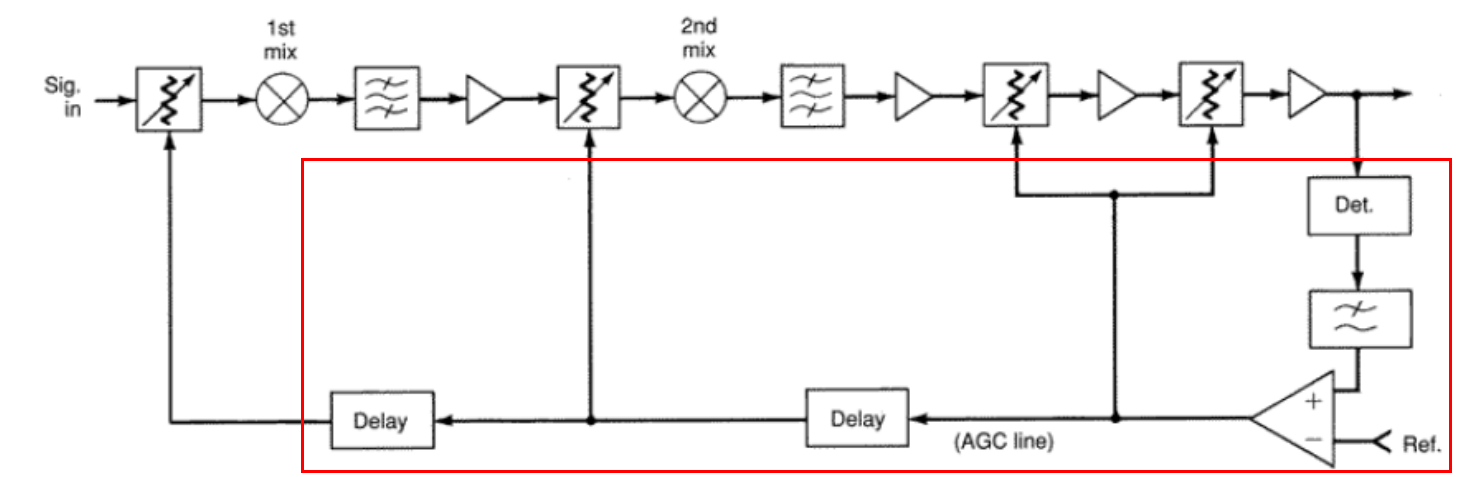
\includegraphics[width=2.5in]{fig/AGC.png}
\caption{Example of receiver AGC, from \cite{AGC_QSL}}
\label{AGC_QSL}
\end{figure}



%\subsection{Variable strength signal} \label{VariableStrength}
%Re-examining the experiments in \Cref{StrongSine} and the disclosed circuit designs, the AGC circuit could have tuned down the signal which might consequently prevented the seed from being biased. If this is the case, then the signal would need to get around the AGC to bias the seed.
%
%\begin{figure}[!t]
%\centering
%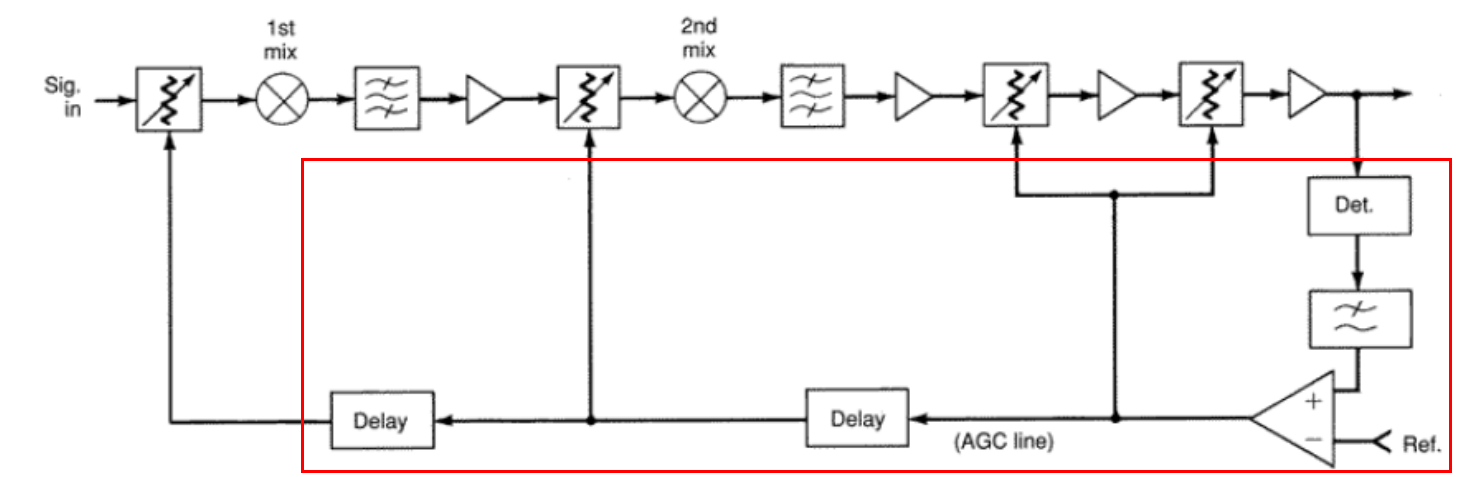
\includegraphics[width=2.5in]{fig/AGC.png}
%\caption{Example of receiver AGC, from \cite{AGC_QSL}}
%\label{AGC_QSL}
%\end{figure}
%
%Although the exact AGC design for CC2538 is unclear, \Cref{AGC_QSL} demonstrates an example of AGC design using 4 Voltage Controlled Amplifiers (VGAs). The output signal is parallelly connected to a detector to estimate the signal strength. The output of detector is compared to a reference voltage and their difference is provided as a feedback to adjust the control voltage of VGAs. To prevent signal distortion caused by abrupt voltage change, such as during a lightning storm, many AGC design adopts an attack time before it adjusts the gain. \cite{AGC} provides a detailed description of different AGC designs. 
% 
%The variable strength signal is therefore designed as an attempt to exploit the delay in AGC adjustments. To be more specifically, the signal is a sine wave at the working frequency which abruptly increases its strength to create a saturation, and then gradually decimates to tune down AGC. 
% 
%The signal can be achieved by multiplying a strong sine wave signal at the carrier frequency to a controlling sawtooth signal. The resulting signal would hopefully to:
%\begin{enumerate}
%	\item Be able to pass the band pass filter.
%	\item Generate bursts that saturates the ADC; therefore bits sampling during the transients will result into predicted bits.
%\end{enumerate}
%
%In our experiments, we used the default frequency $2475MHz$ for the carrier wave. The CC2538 User's Guide\cite{CC2538Manual} stated a programmable register (RFCORE\_XREG\_AGCCTRL3) which allows the user to select the AGC settle timing between 15, 20, 25 and 30 periods with default at 20. In the same document, the description of register RFCORE\_XREG\_RFC\_OBS\_CTRL0 stated that the random bit at both I and Q channels are updated at $8MHz$ which suggests that the receiver may have a sample rate of $16MHz$. Since the controlling signal should be slightly lower than the AGC adjustment frequency, this would give us a sawtooth signal near $0.8MHz$.
 
%Formally, denote the carrier signal $V_C$ as:
%\begin{equation}
%	V_{C}(t) = A\sin(\omega_{C} t)
%\end{equation}
%where $\omega_{C} = 2475MHz$ is the carrier frequency in our case. The signal needs to be strong enough to transiently saturate the ADC when the RF is detecting environmental noise. Assuming an 8 bit ADC and environmental noise at $-92dBm$, $V_{C}$ requires to be theoretically at least $-68dBm$.
%
%We control the amplitude by a sawtooth signal $V_{S}$ denote as:
%\begin{equation}
%	V_{S}(t) = - (\omega_S t \mod 1) + 1
%\end{equation}
%where $\omega_S$ is the frequency of bursts in the signal which is much lower than $\omega_C$ and should be slightly lower than the frequency of AGC adjustments.
%
%The desired signal is $V(t)$ is their product:
%\begin{equation}
%	V(t) = V_C(t)V_S(t)
%\end{equation}
%
%$V(t)$ is hopefully to have two properties:
%\begin{enumerate}
%	\item Being able to pass the band pass filter.
%	\item Generate bursts that saturates the ADC; therefore bits sampling during those period results into predicted bits.
%\end{enumerate}

%The signal source is implemented using Gnu Radio Companion\cite{GRC} with a HackRF One\cite{HackRFOne} directly connected to an OpenMote\cite{OpenMote}. However, no significant bias was reported by the NIST test suite. The exact cause of failure is unknown due to lack of design documentation but one potential reason might be that the period of transient is too short to significantly affect the seed.

\subsection{Strong constant signal} \label{Constant}
We then attempted a strong constant signal. The idea is to treat the whole circuit as a deterministic compression function that maps any $V_{in}$ to $\{0,1\}$. Under this assumption, the same $V_{in}$ should always generate the same $b$, either $0$ or $1$.
In order to achieve constant $V_{in}$ in \Cref{V_in}, $V_s$ needs to be significantly greater than $N$ to suppress its impact in \Cref{RNDOutput}, as any ADC would have only a limited resolution.

For experimental purpose, we have configured three programmable LNAs in the AGC to their maximum gain ($6 + 21 + 9 = 36(dB)$) and has disabled the attenuator in Anti Aliasing Filter (AAF, up to $9dB$). We consider these modifications can be compensated by a strong signal amplifier in practice. The signal source is implemented by Gnu Radio Companion (GRC)\cite{GRC} with HackRF One\cite{HackRFOne}, connected to the target OpenMote through a SMA cable for the best signal strength. \Cref{ConstantSignal} lists the configuration which effectively generates a carrier wave on desired frequency.

\begin{table}[!t]
\caption{GRC Signal Source Configuration}
\label{ConstantSignal}
\centering
\begin{tabular}{|c|c|}
\hline
\textbf{Sample Rate} & 8 MHz             \\ \hline
\textbf{Output Type} & Complex           \\ \hline
\textbf{Waveform}    & Constant \\ \hline
%\textbf{Frequency}   & 2475 MHz          \\ \hline
\textbf{Amplitude}   & 0                 \\ \hline
\textbf{Offset}      & 1                \\ \hline
\textbf{IF Gain}      & [0, 30] dB               \\ \hline
\textbf{Output Voltage Amplitude} & [0,176.0] mV \\ \hline
\end{tabular}
\end{table}

Applying the signal, we observed abnormal 0-runs, i.e. consecutive $0$ bits, appeared in the seeds as we increase IF gain to values above $10dB$. \Cref{IFvsP0} shows how $P(0)$ is biased and \Cref{IFvsN0} shows the average number of bits of longest 0-runs in each seed. We can see that the bias has reached its peak at $\text{IF\_Gain} = 22dB$ in both figures. At such gain $27.709\%$ of the 128 bit seeds have longest 0-runs over $64$ bits. It is not a surprise to see the sampled seeds have failed nearly all tests in the NIST test suite, indicating they have been strongly biased by our signal. We cannot determine the exact cause of bias decrease for IF Gain over $22$dB due to lack of circuit design, but one potential caused might be the distortion under strong signal strength.

\begin{figure*}[!t]
\centering
\subfloat[$P(0)$ to IF Gain]{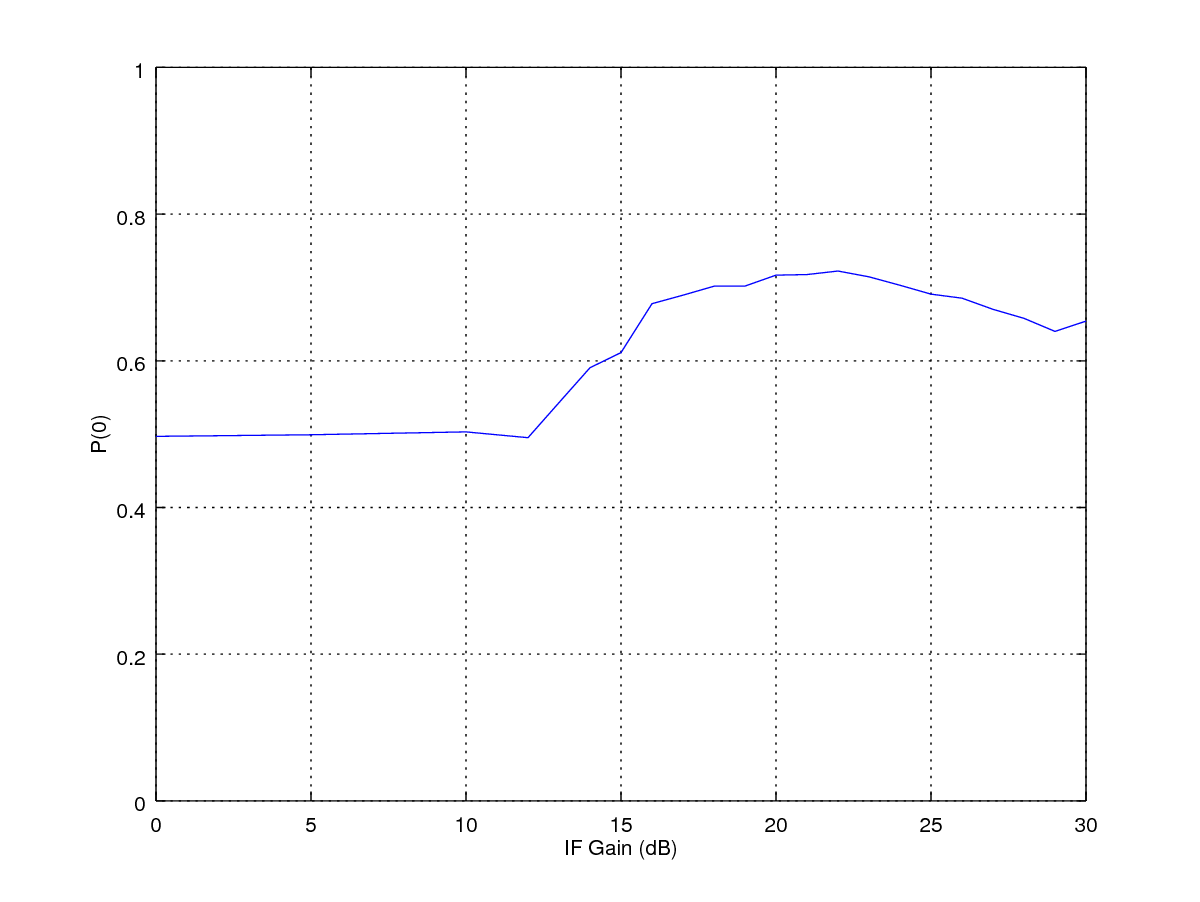
\includegraphics[width=2.5in]{fig/if_vs_P0_new.png}
\label{IFvsP0}}
\hfil
\subfloat[Average longest 0-runs in each seed to IF Gain]{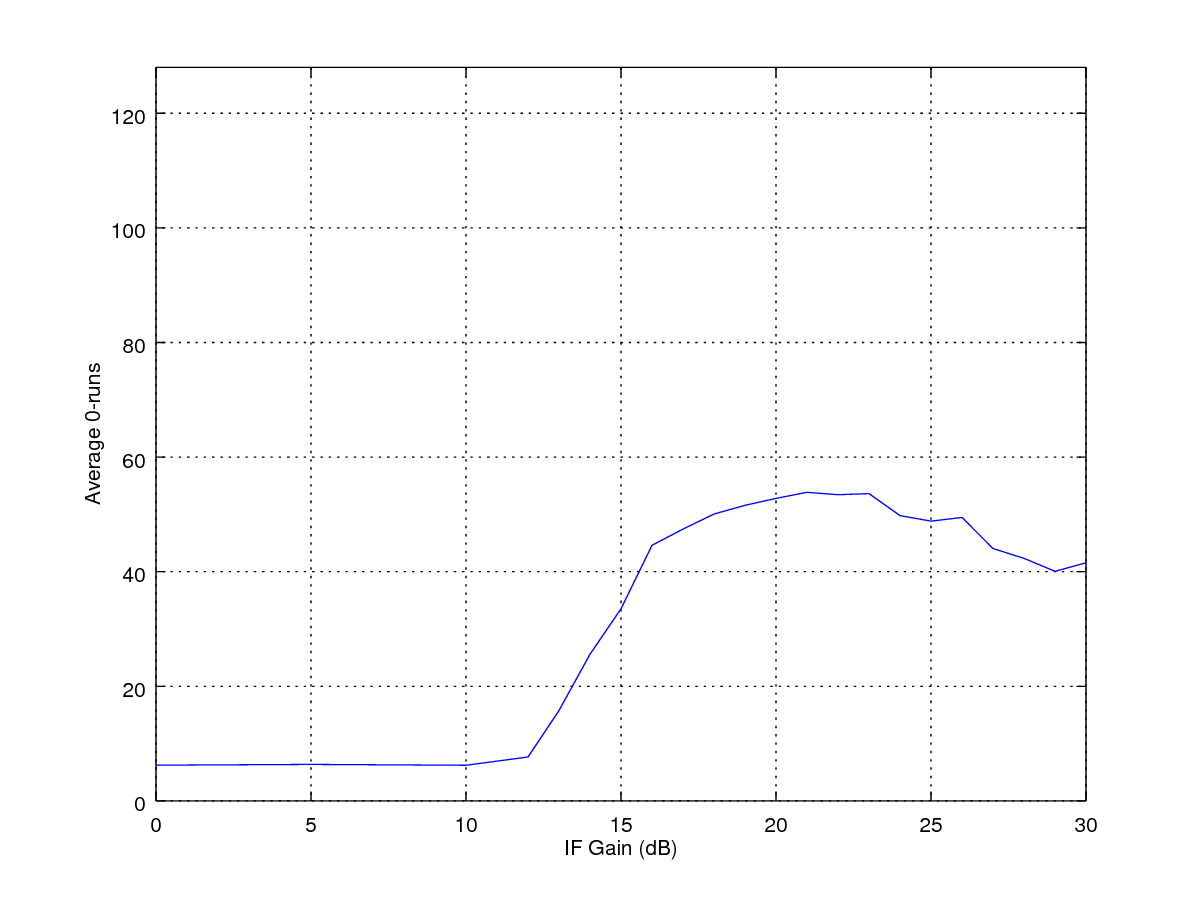
\includegraphics[width=2.5in]{fig/if_vs_N0_new.png}
\label{IFvsN0}}
\caption{Biased Seed on OpenMote. Signal source amplitude from $19.5$mV (10dB), $76.0$mV(22dB) to $176.0$mV (30dB).}
\label{ConstantSignalBiased}
\end{figure*}

We also re-applied the signal to the same OpenMote we previously used in the strong sine wave signal experiments. A even stronger bias is observed as shown in \Cref{StronglyBiased}, with $17.820\%$ of the seeds ended in 128 consecutive $0$ bits. This may be caused by the strong sine wave signal in the previous experiments which permanently biased the device. We therefore restored its AGC configuration to default and re-ran the NIST test suite but the sampled seed passed all tests as before. We also tested using example applications provided by Contiki and found no malfunctioning on the device. The permanent bias does not seem to affect the device under normal operational status and can only be triggered by the constant signal. This leads to a very dangerous attack where devices could be primed in such a way that they remain functional under normal operating conditions, and eventually `activated' via supplying the activation signal upon which they are unable to produce random numbers and hence all DTLS connections would be completely insecure. We were able to replicate this attack on brand new devices with factory settings.

\begin{figure*}[!t]
\centering
\subfloat[$P(0)$ to IF Gain]{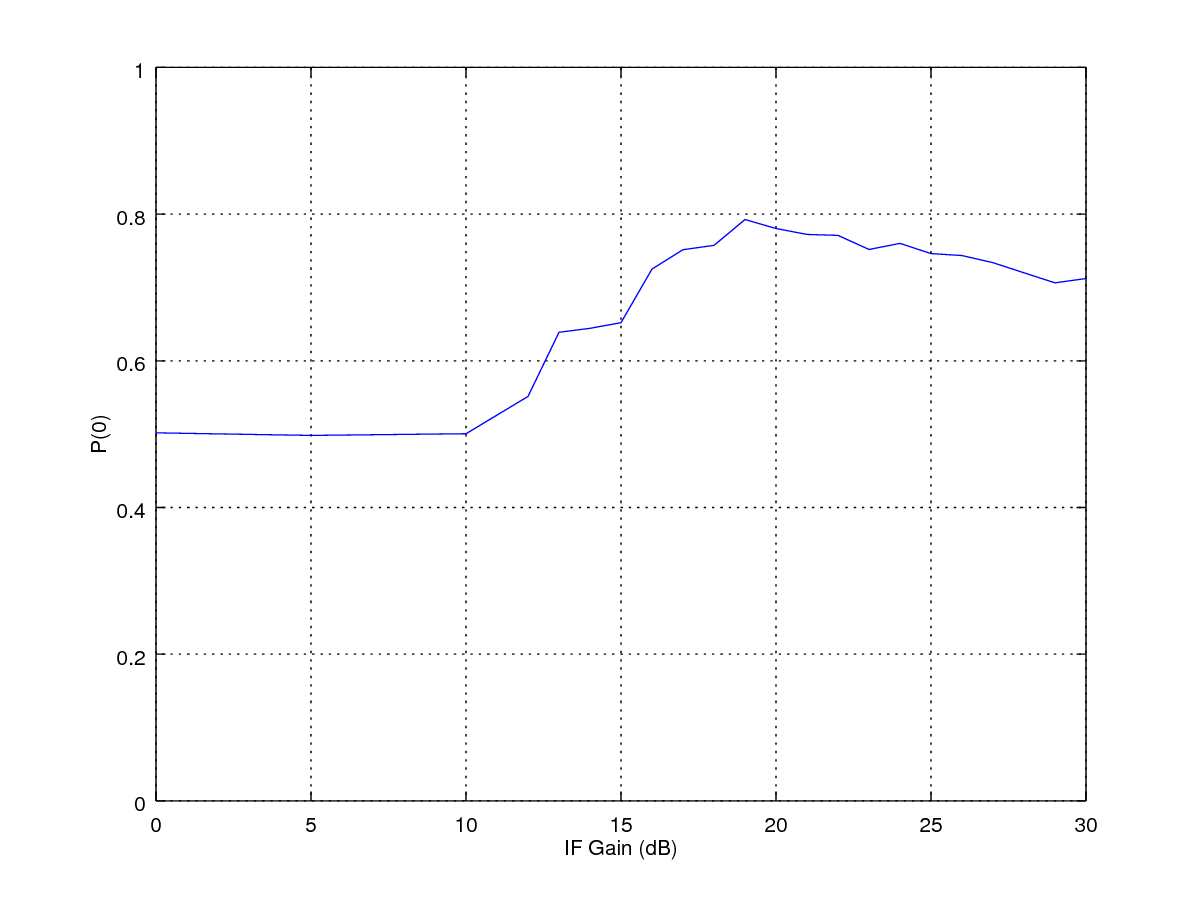
\includegraphics[width=2.5in]{fig/if_vs_P0.png}}
\hfil
\subfloat[Average longest 0-runs in each seed to IF Gain]{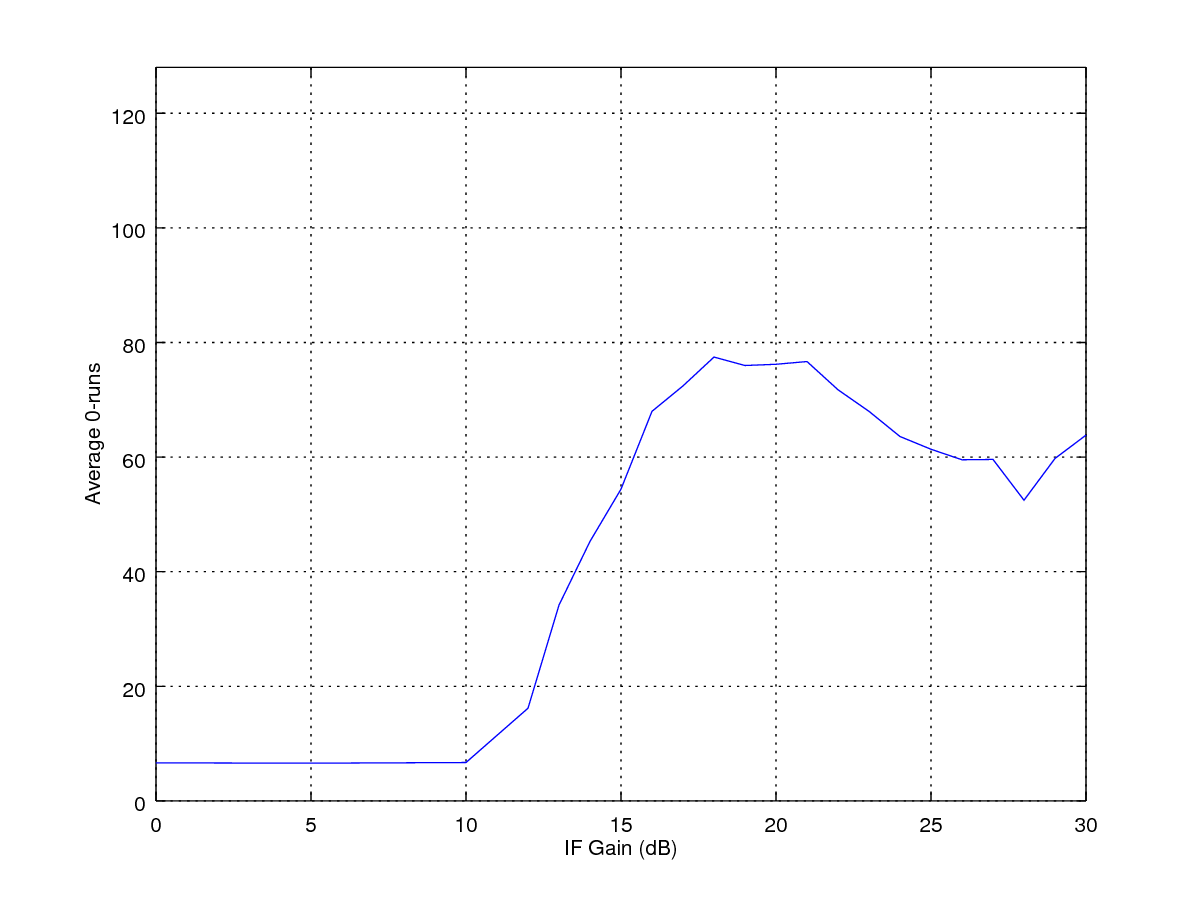
\includegraphics[width=2.5in]{fig/if_vs_N0.png}}
\caption{Biased Seed on OpenMote used in previous experiments. Signal source amplitude from $19.5$mV (10dB), $76.0$mV(22dB) to $176.0$mV (30dB).}
\label{StronglyBiased}
\end{figure*}

%Again due to lack of design documentation we can not explain how exactly the bias is triggered by the signal. Nevertheless our experiments have demonstrated that sampling seed using RF noise could potentially be biased by jamming signal and hence potentially breaching any cryptographic protocol relies on its randomness.